\documentclass{beamer}

% This file is a solution template for:

% - Giving a talk on some subject.
% - The talk is between 15min and 45min long.
% - Style is ornate.

% Copyright 2004 by Till Tantau <tantau@users.sourceforge.net>.
%
% In principle, this file can be redistributed and/or modified under
% the terms of the GNU Public License, version 2.
%
% However, this file is supposed to be a template to be modified
% for your own needs. For this reason, if you use this file as a
% template and not specifically distribute it as part of a another
% package/program, I grant the extra permission to freely copy and
% modify this file as you see fit and even to delete this copyright
% notice. 

%MATH
\newcommand{\vectornorm}[1]{\left|\left|#1\right|\right|}
\newcommand{\spectralnorm}[1]{\left|\left|#1\right|\right|_{2}}

\mode<presentation>
{
	\usetheme{Oxygen}
  %\usetheme{Madrid}
	% or ...
  %\usecolortheme{whale}
  %\setbeamercovered{transparent}
  % or whatever (possibly just delete it)
}


\usepackage[english]{babel}
% or whatever
\usepackage{amssymb}
\usepackage{amsmath}

\usepackage[utf8x, utf8]{inputenc}
% or whatever

\usepackage{times}
\usepackage[T1]{fontenc}
\usepackage{color}
\usepackage{natbib}
\usepackage[official]{eurosym}
\newcommand{\spacing}{1.5}

\usepackage{multimedia}
\usepackage[bigfiles]{media9}
\addmediapath{videos}
\usepackage{hyperref}
% Or whatever. Note that the encoding and the font should match. If T1
% does not look nice, try deleting the line with the fontenc.
\usepackage{thumbpdf}
\usepackage{wasysym}
%\usepackage{ucs}
\usepackage{pgf,pgfarrows,pgfnodes,pgfautomata,pgfheaps,pgfshade}
\usepackage{verbatim}
\usepackage{colortbl}
\usepackage{ragged2e} %Justify
\usepackage{booktabs} %% Rules separation for tables (Top, mid, bottom)

%For the pictures
\usepackage{epic}\setlength{\unitlength}{1cm}
\usepackage{eepic}\setlength{\unitlength}{1cm}
\usepackage{longtable}
\usepackage{array}
\usepackage{multicol}

%Animations
\usepackage{animate}
\usepackage{pgfplots}
\usepackage{tikz}
\usetikzlibrary{	
	calc
}

\setbeamertemplate{navigation symbols}{}%remove navigation symbols

\definecolor{greenBlue_pres}{HTML}{16A085}

\title[TITLE]
{\Large TITLE}

\author[AUTHOR] % (optional, use only with lots of authors)
{AUTHOR}
% - Use the \inst{?} command only if the authors have different
%   affiliation.
\institute
{\small INSTITUCIÓN}

%\date[\today] % (optional)
%{\today}
\date[DATE] 
{DATE}

%\institute[IES-UPM] % (optional, but mostly needed)
%{\textbf{Máster de Domótica y Hogar Digital} \\ \vspace{0.5cm} IES-UPM}

\subject{Talks}
% This is only inserted into the PDF information catalog. Can be left
% out. 



% If you have a file called "university-logo-filename.xxx", where xxx
% is a graphic format that can be processed by latex or pdflatex,
% resp., then you can add a logo as follows:

%\pgfdeclareimage[height=0.5cm]{university-logo}{figs/ies.eps}
%\logo{\pgfuseimage{university-logo}}

%\logo{
\includegraphics[height=1cm]{figs/ies.eps} \hspace{0.10cm} \vspace{0.10cm}}


% Delete this, if you do not want the table of contents to pop up at
% the beginning of each subsection:
\AtBeginSection[]
{
  \begin{frame}
    \frametitle{~}
    \tableofcontents[currentsection]
  \end{frame}
}

\AtBeginSection[]
{
  \frame<handout:0>
  {
    \frametitle{Contents}
    \tableofcontents[currentsection,hideallsubsections]
  }
}

\AtBeginSubsection[]
{
  \frame<handout:0>
  {
    \frametitle{Contents}
    \tableofcontents[sectionstyle=show/hide,subsectionstyle=show/shaded/hide]
  }
}

\newcommand<>{\highlighton}[1]{%
  \alt#2{\structure{#1}}{{#1}}
}

\newcommand{\icon}[1]{\pgfimage[height=1em]{#1}}


\begin{document}
\def\newblock{\hskip .11em plus .33em minus .07em}
\graphicspath{{../figs/}}

%------Titulo------%
\begin{frame}[plain]
  \vspace{0.75cm}
	\titlepage
  \vspace{-0.5cm}
  \begin{center}
    \begin{tabular}{cc}
      \includegraphics[width=3.0cm]{rblb.eps} & 
      
\includegraphics[width=3.75cm]{etsit.eps} \\
    \end{tabular}
  \end{center}
\end{frame}

%+++++++++++++++++++++++++++++++++++++++++++++++++++++++++++++++++++++++++%
\section{Introduction}

%------------%
\begin{frame}
	\frametitle{Golden Rule}
	\begin{center}	
	Generation $=$ Consumption, $\forall t$\\[1.0cm]
	
\includegraphics[width=7cm]{electricalMatching.eps}\\[0.5cm]
	Origin of major problems...
	\end{center}
\end{frame}

%------------%
\begin{frame}
	\frametitle{Electric system}
	\begin{center}	
    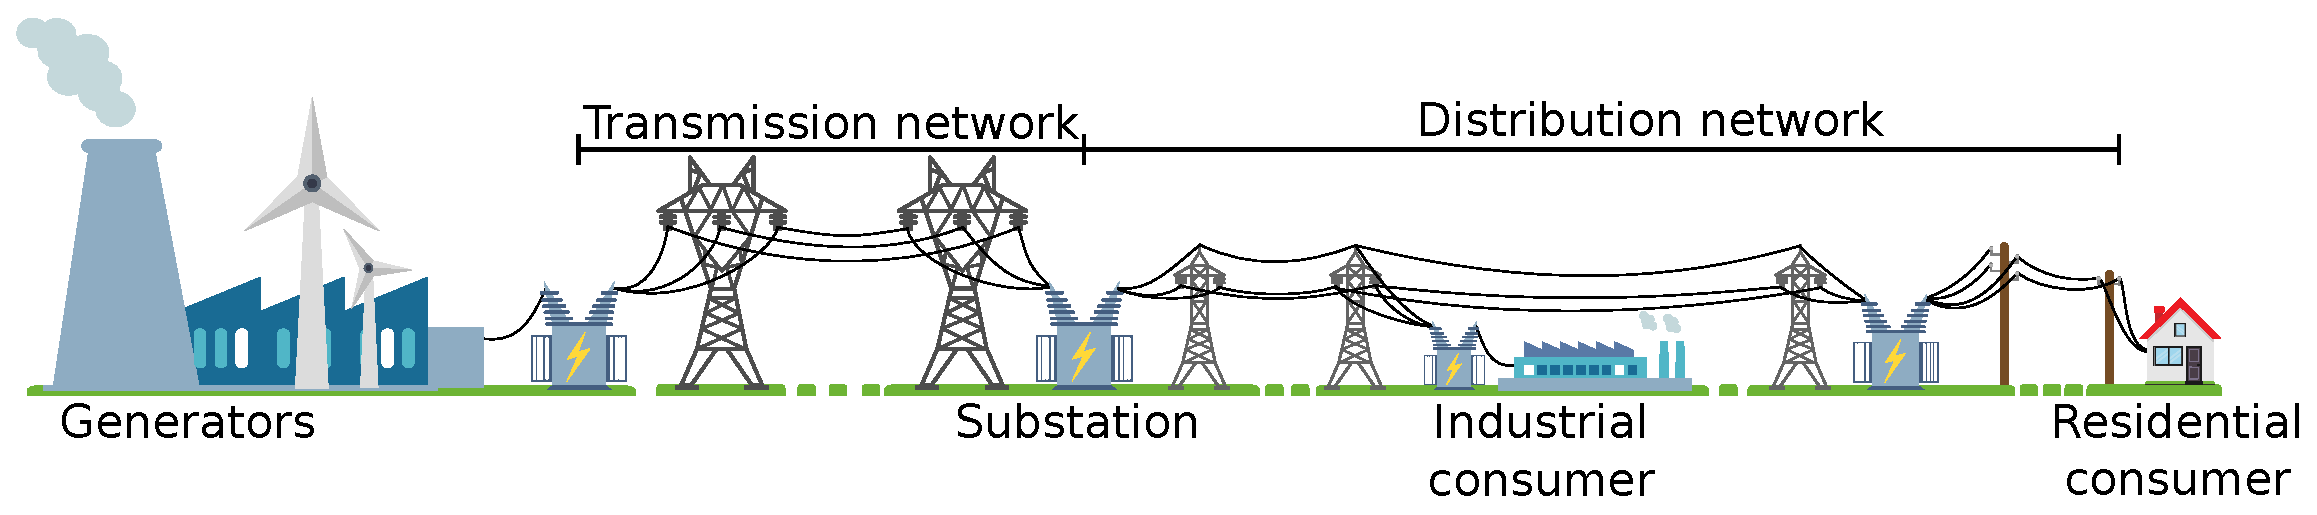
\includegraphics[width=11cm]{grid_sketch.eps}
	\end{center}
	\begin{itemize}
	  \item{{\bf Generators}: }produce electric power from primary sources.
	  \item{{\bf Transmission network}: }from power plants to substations.
	  \item{{\bf Substations}: }power conditioning and safety mechanism.
	  \item{{\bf Distribution network}: }from substations to consumers.
	  \item{{\bf Consumption}: }transforms electric power into work.
	\end{itemize}
\end{frame}

%------------%
\begin{frame}
	\frametitle{Problems}
  \begin{center}
    {\bf Generation must adapt to consumption, but ...}\\ 
    \begin{columns}
      \hspace{0.5cm}
      \column{2.5cm}
      \begin{center}
        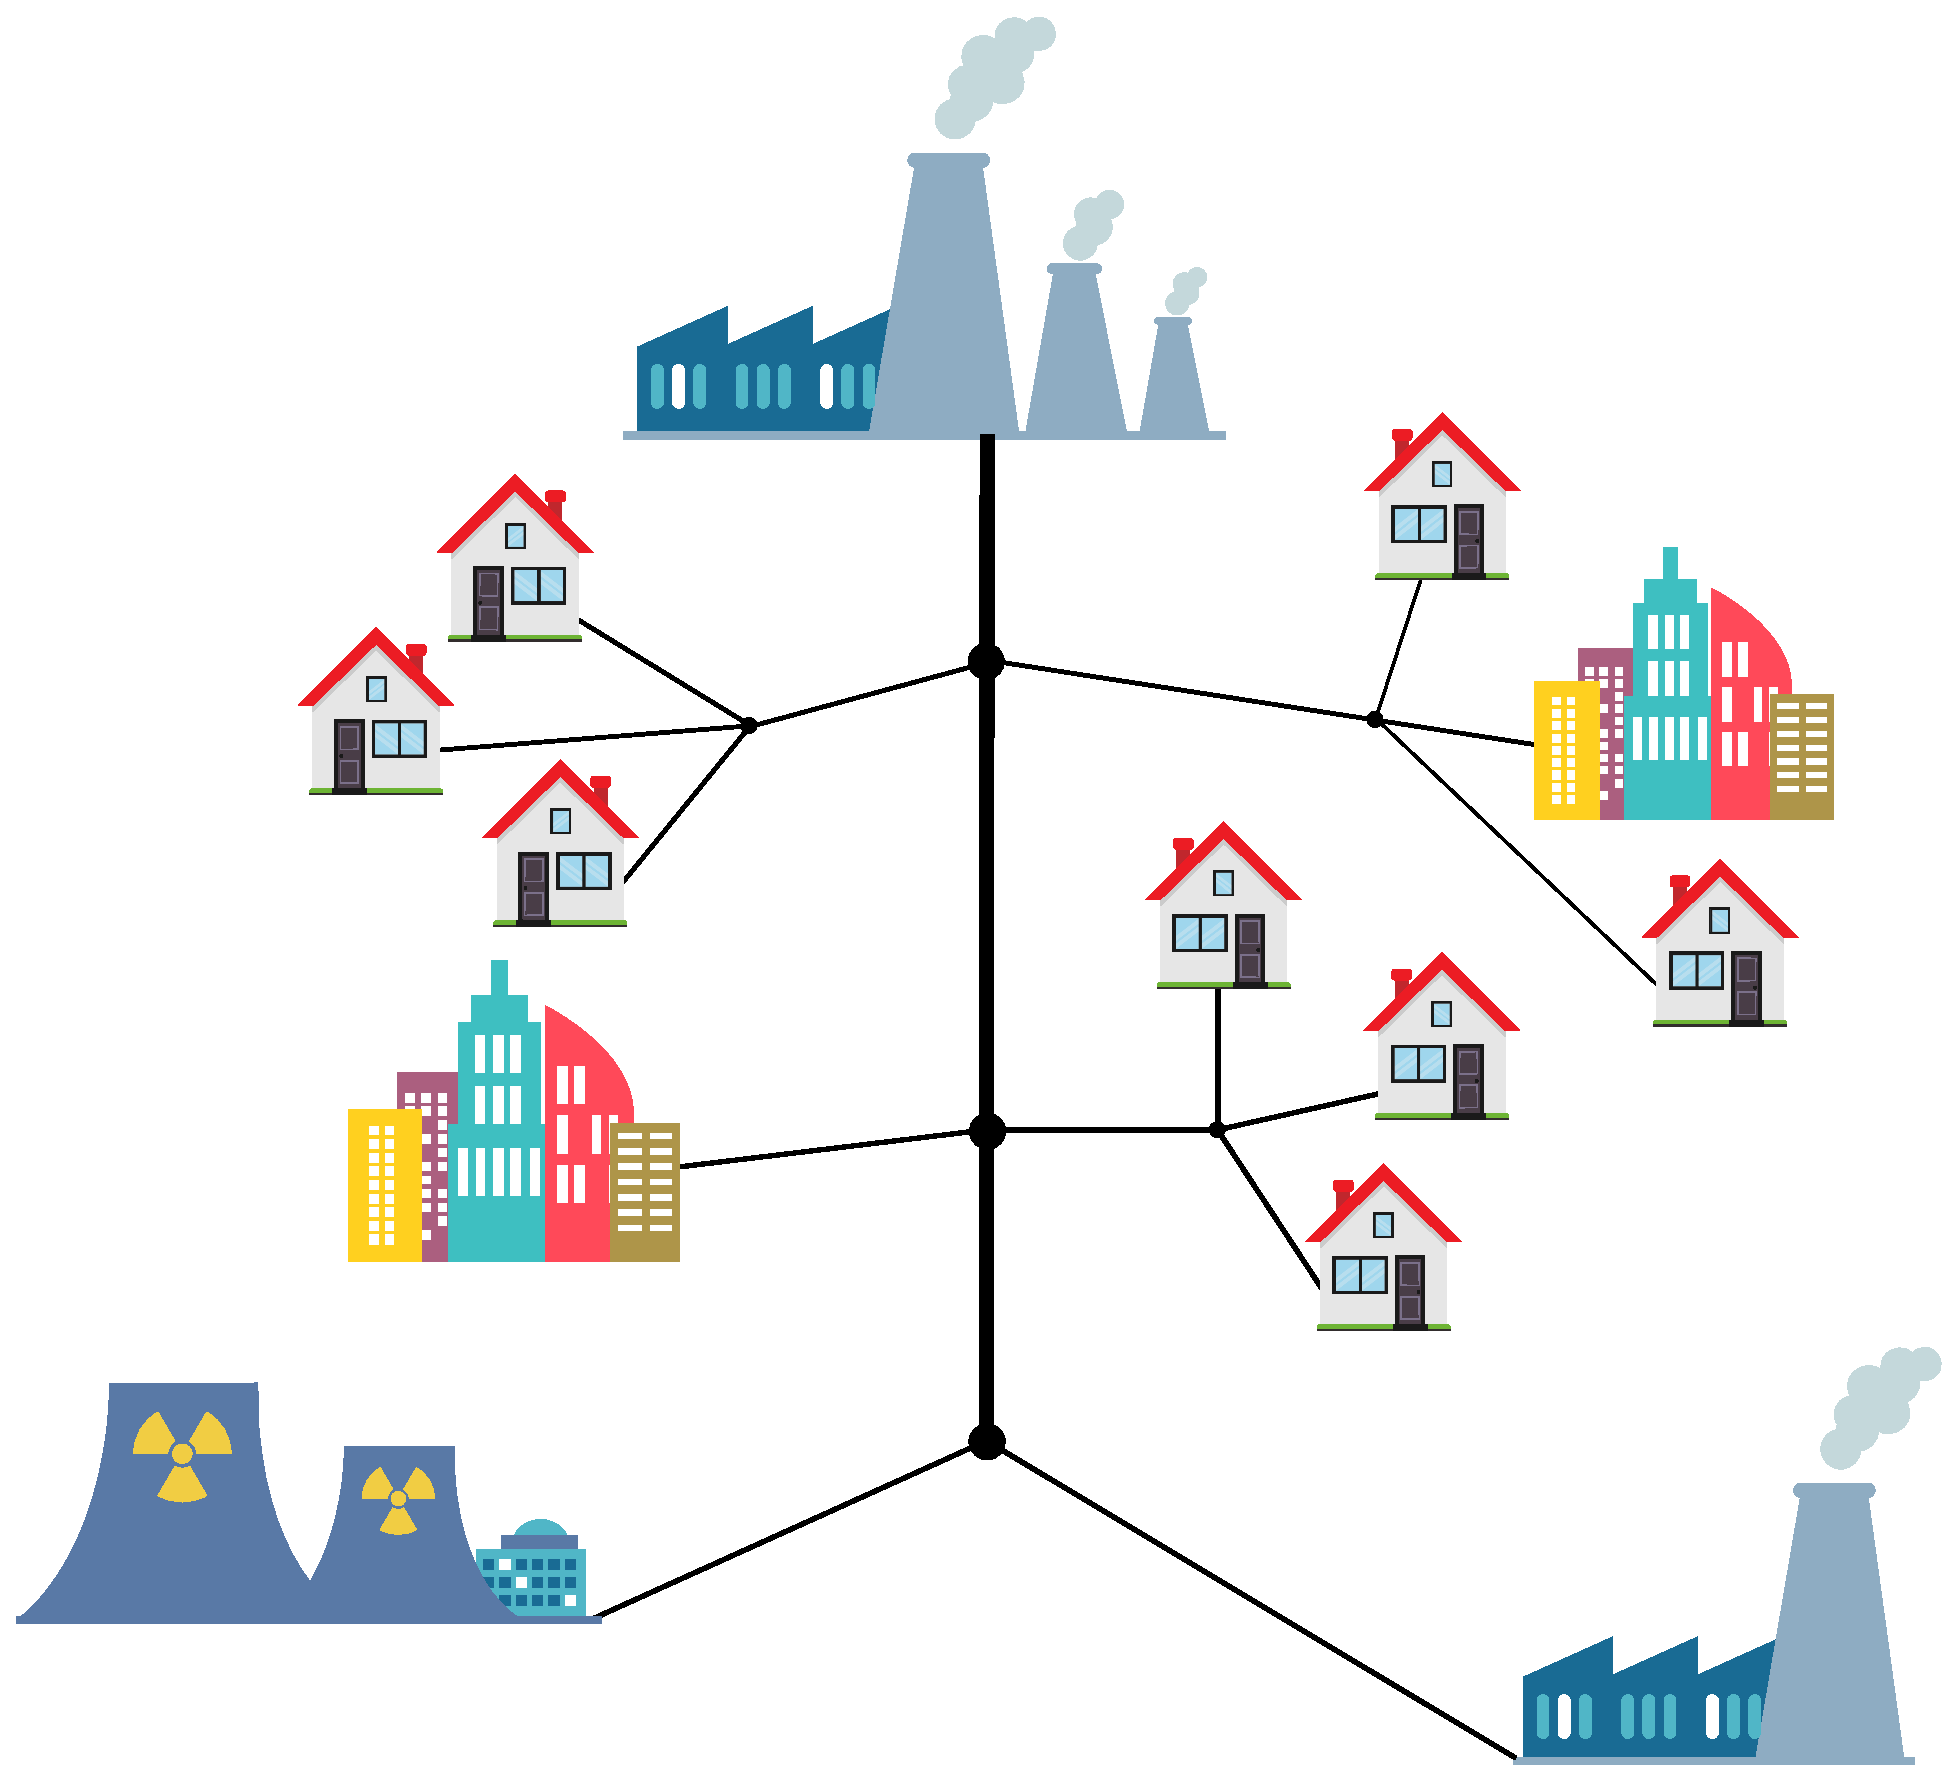
\includegraphics[width=3.00cm]{oldGenerationGrid.eps}
      \end{center}
      \column{7cm}
      \begin{itemize}
        \item {\bf Grid:}
        \begin{itemize}
          \item Centralized system
          \item Ageing infrastructure 
          \item Generation far from consumption 
          \item Losses $\longrightarrow$ Efficiency $\downarrow \downarrow$
        \end{itemize} 
      \end{itemize} 
    \end{columns} 
    \begin{columns}
      \column{5cm}
      \begin{itemize}
        \item {\bf Consumption:}
        \begin{itemize}
          \item High variability
          \item High responsiveness
          \item System stress
          \item Grid oversizing %$\longrightarrow$ generation $+$ transport
        \end{itemize} 
      \end{itemize} 
      \column{4cm}
      \begin{flushright}
        \hspace{-2.5cm}
        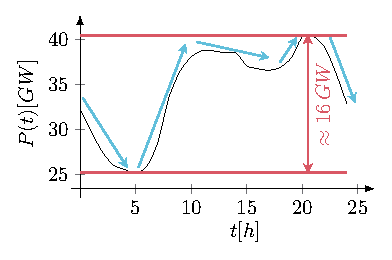
\includegraphics[width=4.5cm]{gridVariability.eps}
      \end{flushright}
    \end{columns} 
  \end{center}
\end{frame}

%------------%
\begin{frame}
  \frametitle{Solution(I): Evolution of the grid}
	\begin{center}	
	  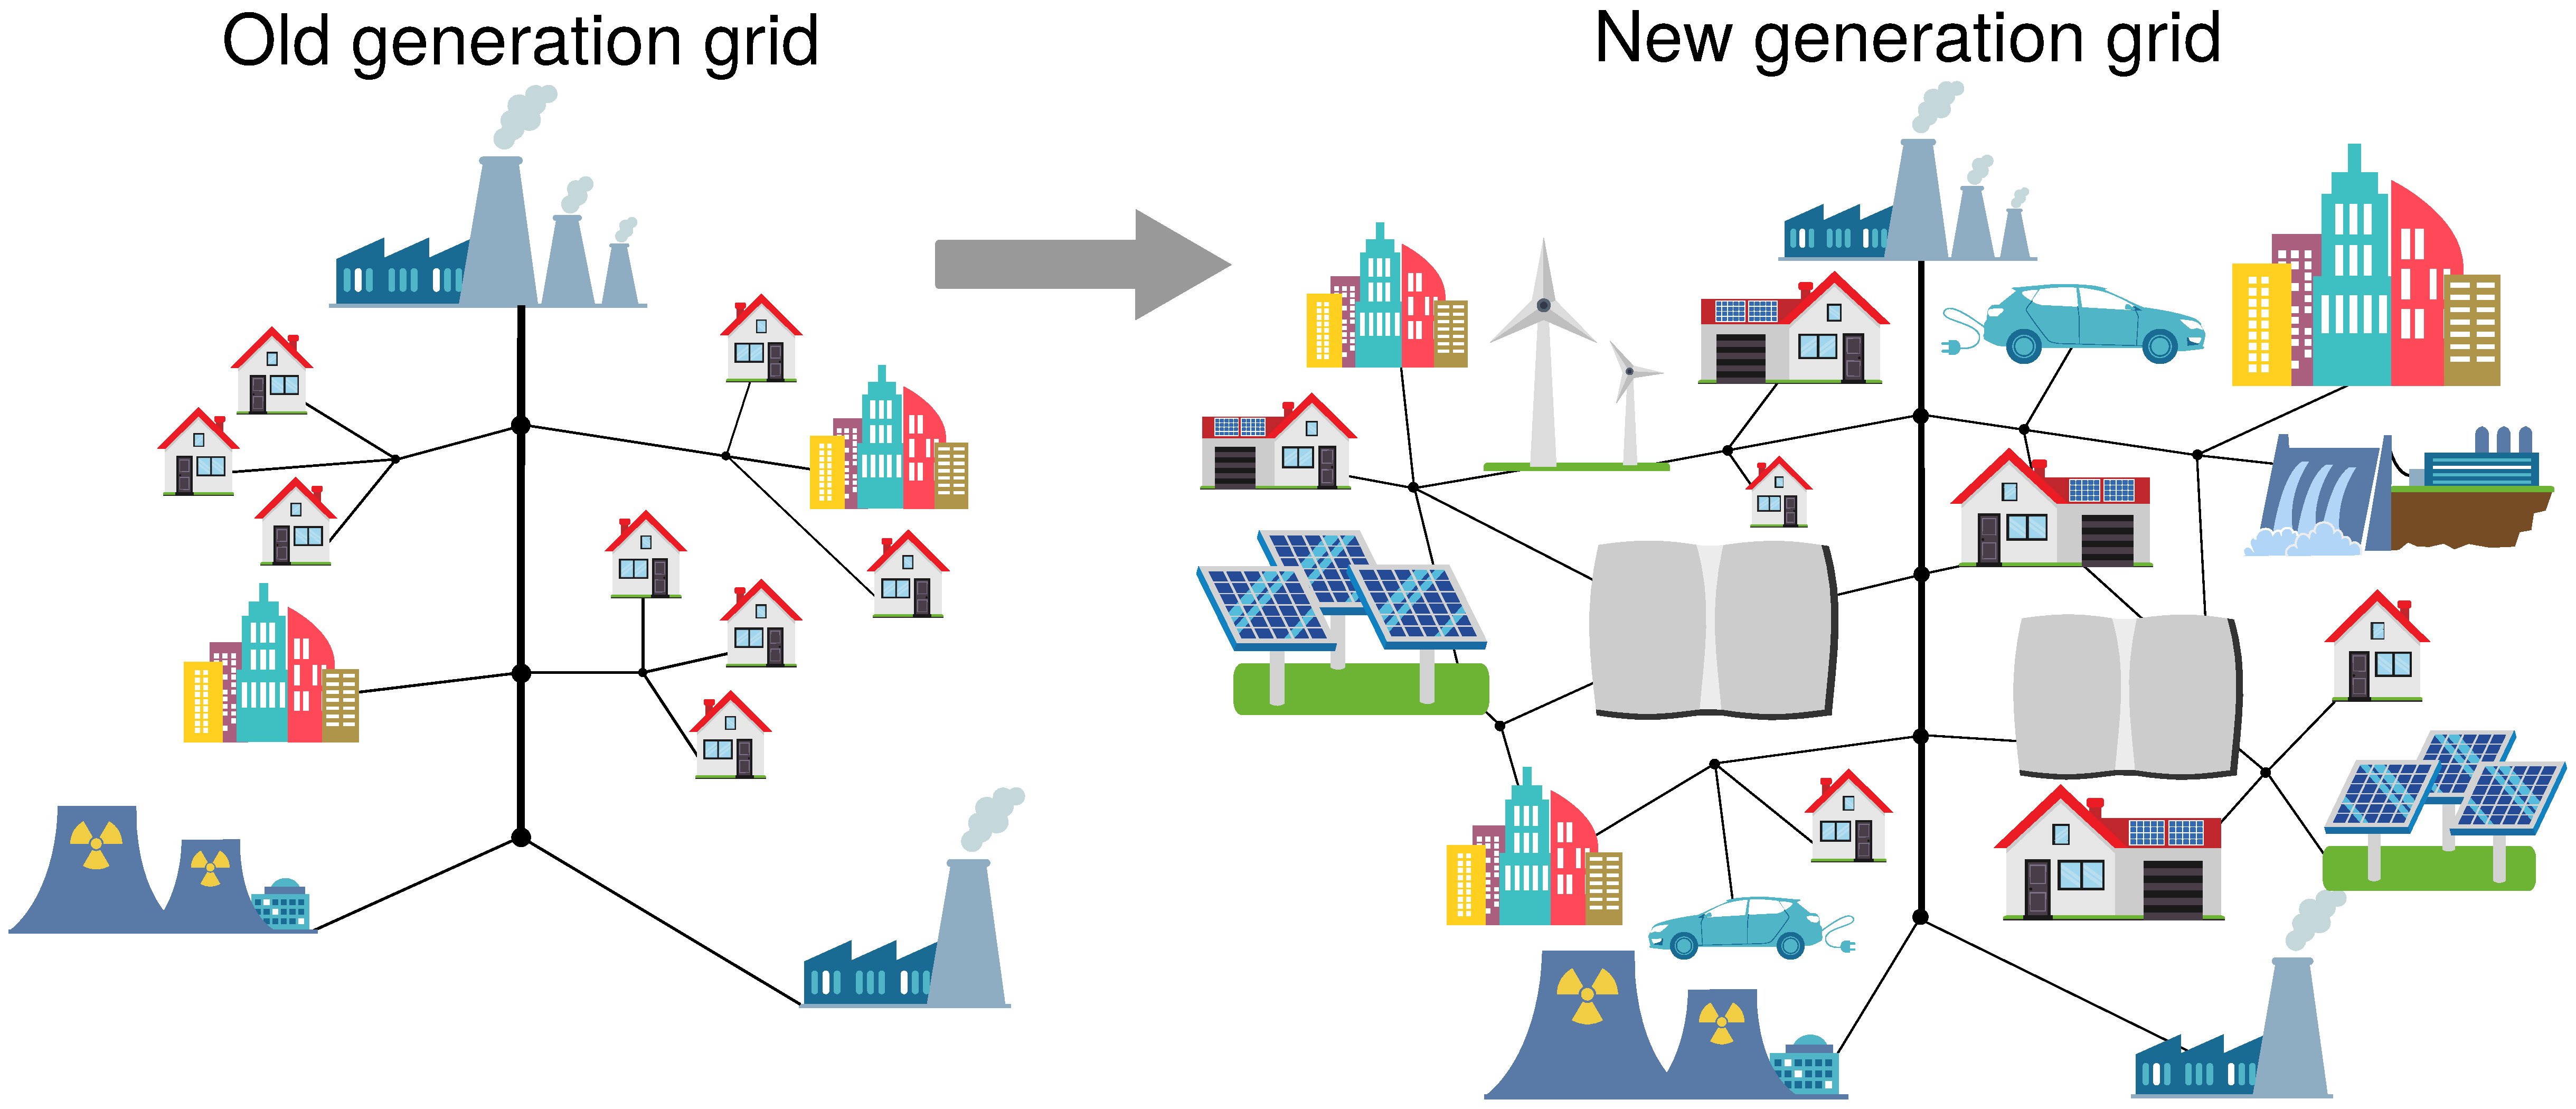
\includegraphics[width=11cm]{gridGeneration.eps}
    \begin{columns}
      \column{4cm}
        \centering
        \begin{itemize}
          \item Centralized
          \item $\downarrow$ Efficiency 
          \item $\downarrow$ Communication 
        \end{itemize}
      \column{4cm}
      \begin{itemize}
        \item Distributed
        \item $\uparrow$ Integration
        \item $\uparrow$ Participation
      \end{itemize} 
    \end{columns} 
	\end{center}
\end{frame}

%------------%
\begin{frame}
  \frametitle{Solution(II): Smart Grid}
	\begin{center}	
	  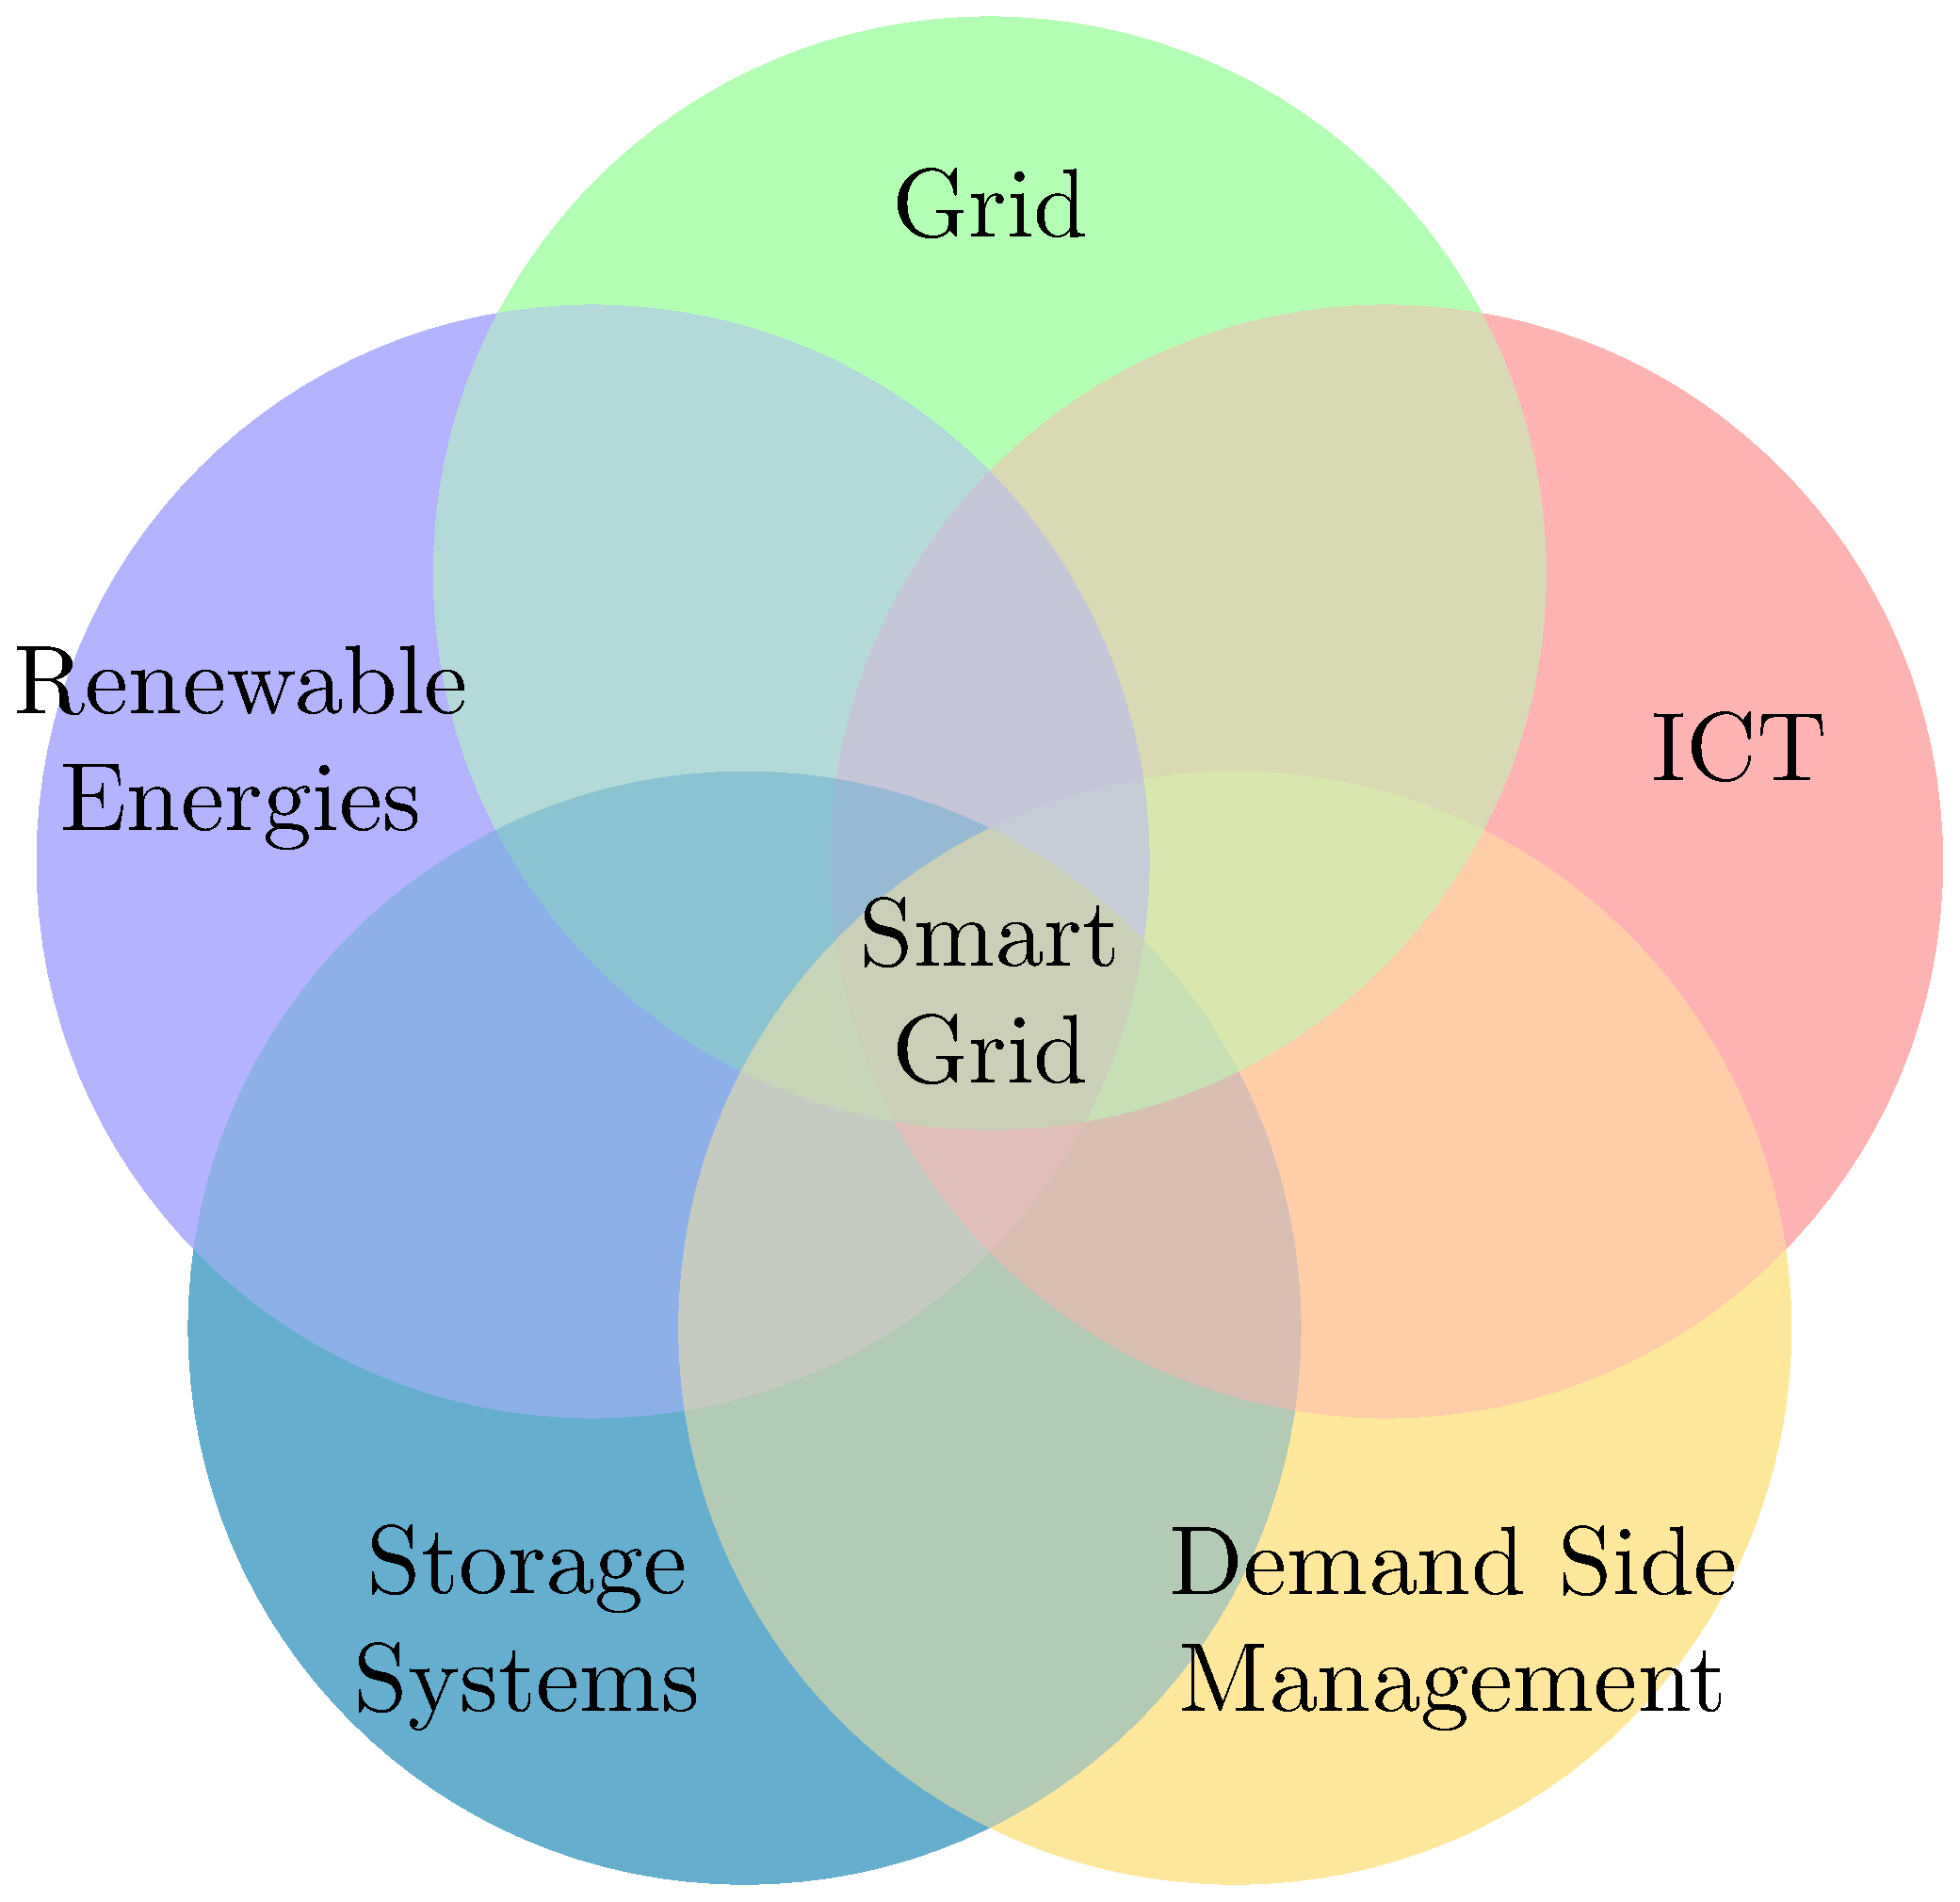
\includegraphics[width=4.75cm]{sgConvergency.eps}
    \begin{block}{Definition}
      \small
      An electricity network that uses communication technologies to coordinate the needs and capabilities of all grid members to operate efficiently, minimising costs and environmental impacts while maximising reliability, resilience and stability.
    \end{block}
	\end{center}
\end{frame}

%------------%
\begin{frame}
  \frametitle{Variability reduction: DSM}
  \begin{center}	
	  \input{../animations/demandSmooth.code}
  \end{center}
\end{frame}

%------------%
\begin{frame}
  \frametitle{Thesis Aim}
  \begin{center}	
    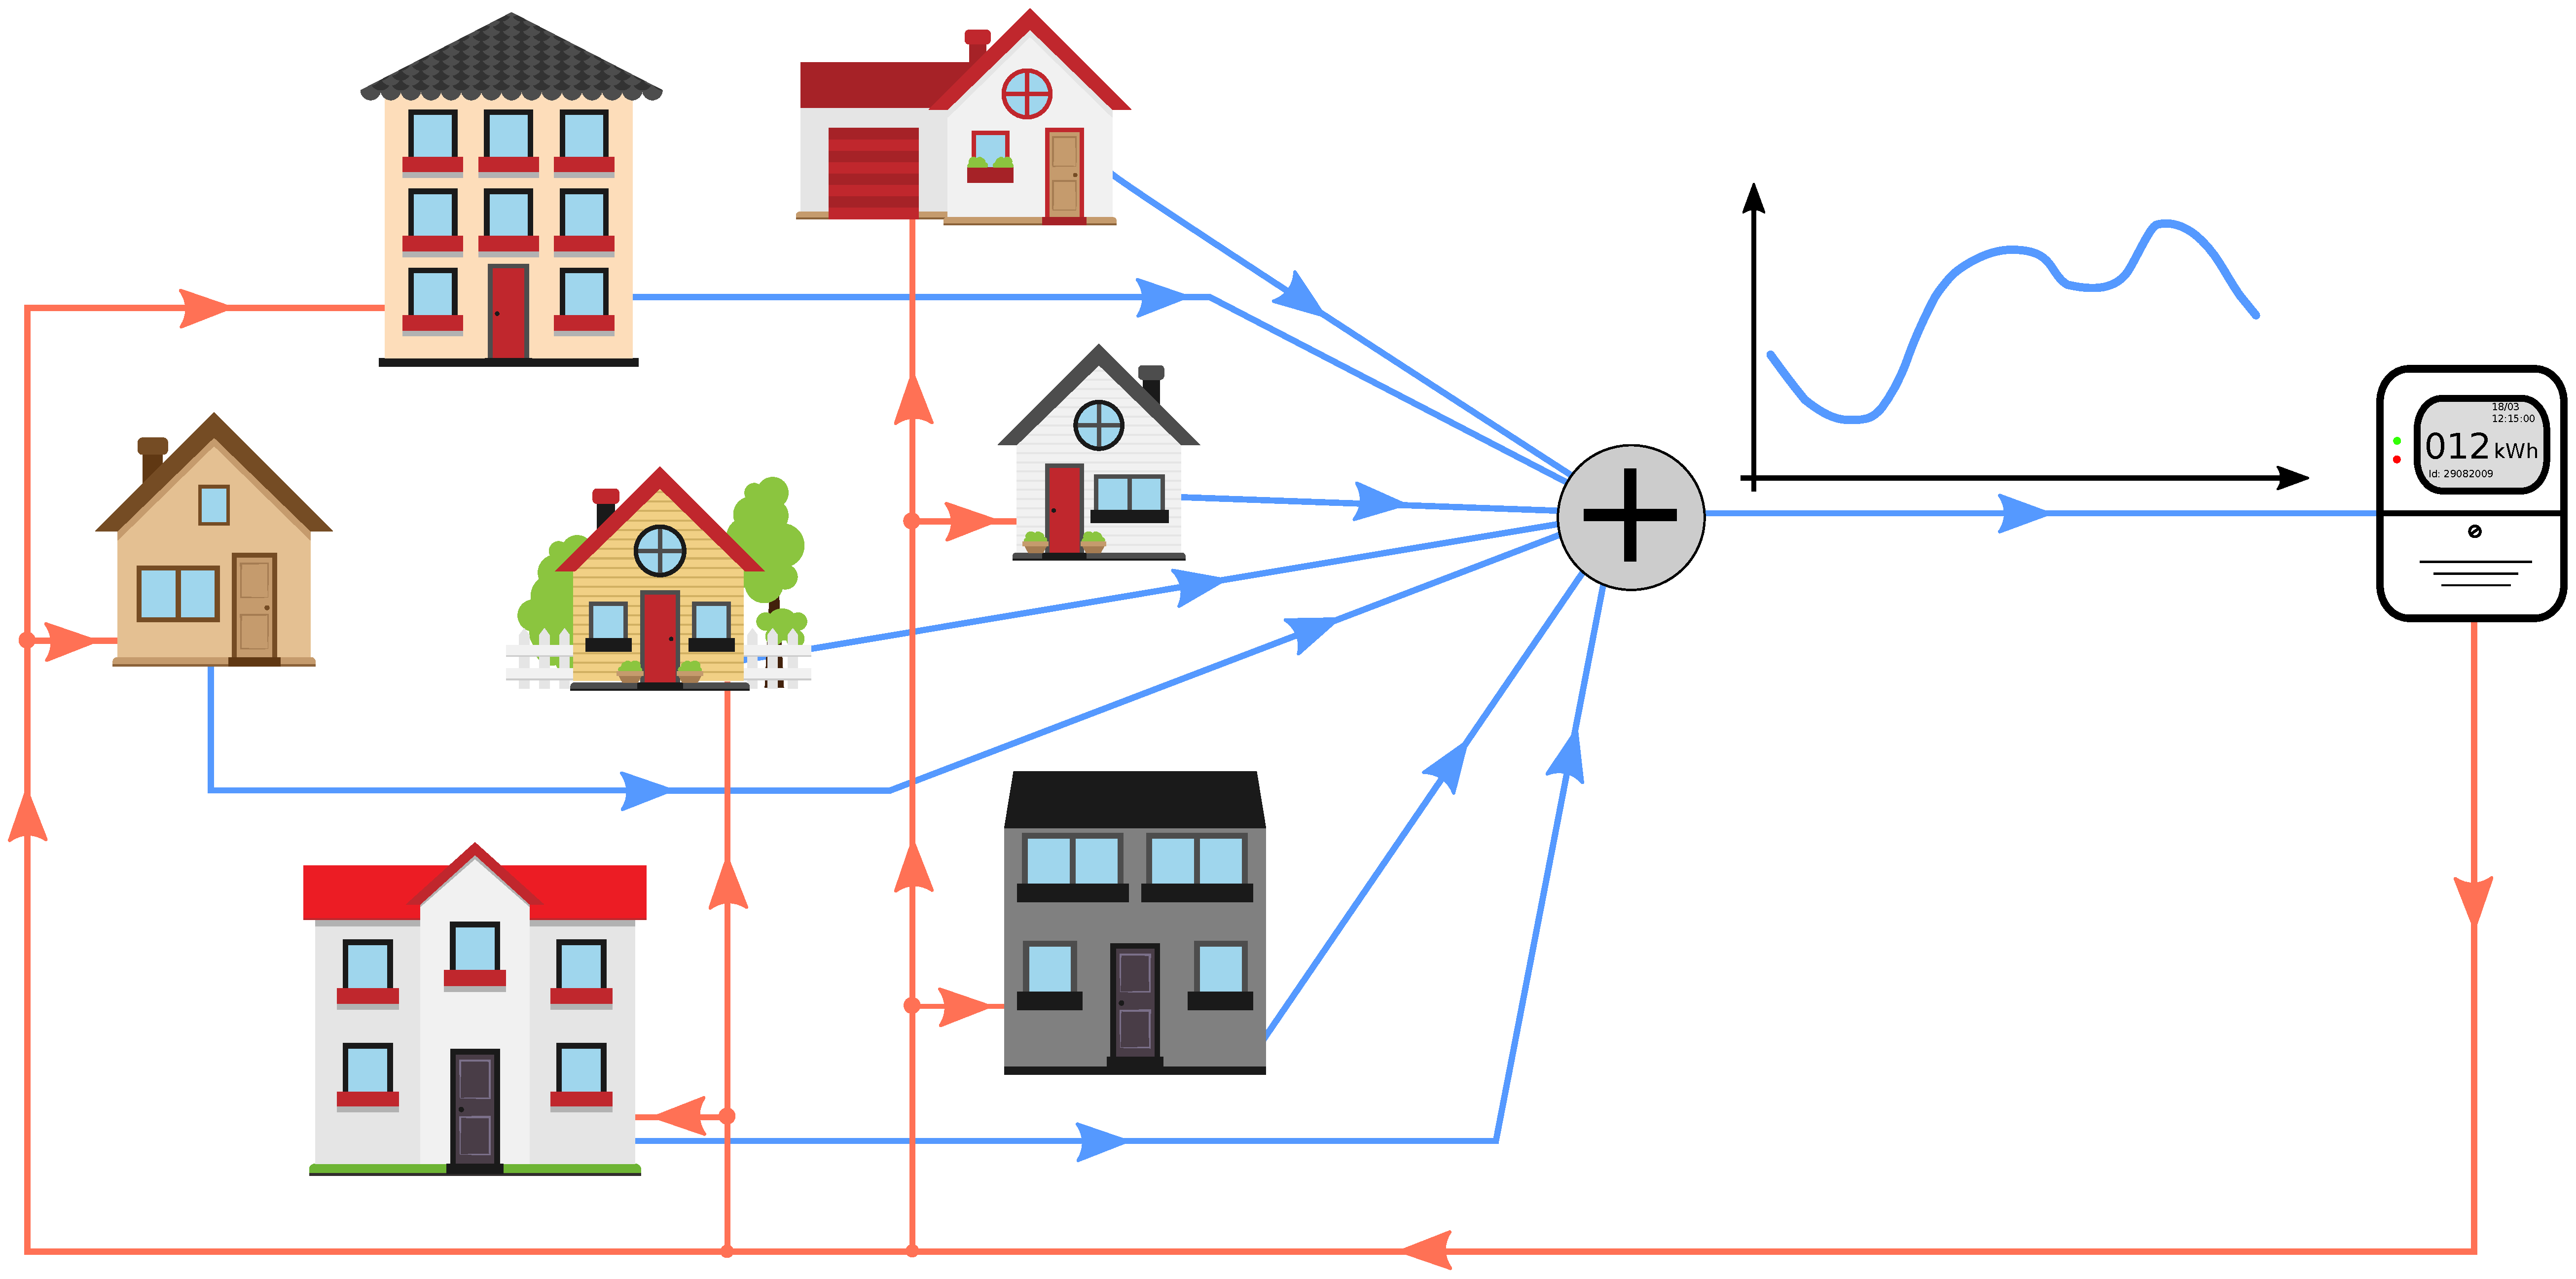
\includegraphics[width=8cm]{objEnv.eps}
  \end{center}
  \vspace{-0.5cm}
  \begin{block}{Objective}
    {\justify
    Development of an adaptive algorithm to manage the consumption of a collective of individuals with the presence of distributed energy resources (PV + local storage).\\
    The algorithm enhances the efficiency of a grid by reducing the variability of the aggregated consumption.}
  \end{block}
\end{frame}

%%%%%%%%%%%%%%%%%%%%%%%%%%%%%%%%%%%%%%%%%%%%%%%%%%%%%%%%%%%%%%%%%%%%%%%%%%%%
\section{Conclusions}

%------------%
\begin{frame}
	\frametitle{ Conclusions }
\end{frame}

%------------%
\begin{frame}
	\frametitle{ Questions }
	\begin{center}
      
\includegraphics[width=4.5cm]{doubts_blue.eps}
      %
\includegraphics[width=4.5cm]{doubts_green.eps}
	\end{center}	
\end{frame}

%------------%
\begin{frame}
  \frametitle{}	
	\begin{center}
      
\includegraphics[width=8.5cm]{thanks.eps}
	\end{center}	
\end{frame}

\end{document}
